\documentclass[12pt]{article}
% \usepackage[top=1in,left=1in, right = 1in, footskip=1in]{geometry}
\usepackage[top=1in,footskip=1in]{geometry}

\usepackage{graphicx}
\usepackage{xspace}
%\usepackage{adjustbox}

\usepackage{multirow}
\usepackage{booktabs}

\usepackage{pdflscape}

\usepackage{grffile}

\newcommand{\comment}{\showcomment}
%% \newcommand{\comment}{\nocomment}

\newcommand{\showcomment}[3]{\textcolor{#1}{\textbf{[#2: }\textsl{#3}\textbf{]}}}
\newcommand{\nocomment}[3]{}

\newcommand{\jd}[1]{\comment{cyan}{JD}{#1}}
\newcommand{\swp}[1]{\comment{magenta}{SWP}{#1}}
\newcommand{\bmb}[1]{\comment{blue}{BMB}{#1}}
\newcommand{\djde}[1]{\comment{red}{DJDE}{#1}}

\newcommand{\eref}[1]{Eq.~(\ref{eq:#1})}
\newcommand{\fref}[1]{Fig.~\ref{fig:#1}}
\newcommand{\Fref}[1]{Fig.~\ref{fig:#1}}
\newcommand{\sref}[1]{Sec.~\ref{#1}}
\newcommand{\frange}[2]{Fig.~\ref{fig:#1}--\ref{fig:#2}}
\newcommand{\tref}[1]{Table~\ref{tab:#1}}
\newcommand{\tlab}[1]{\label{tab:#1}}
\newcommand{\seminar}{SE\mbox{$^m$}I\mbox{$^n$}R}

\usepackage{amsthm}
\usepackage{amsmath}
\usepackage{amssymb}
\usepackage{amsfonts}
\usepackage[utf8]{inputenc} % make sure fancy dashes etc. don't get dropped

\usepackage{lineno}
\linenumbers

\usepackage[pdfencoding=auto, psdextra]{hyperref}

\usepackage{natbib}
\bibliographystyle{chicago}
\date{\today}

\usepackage{xspace}
\newcommand*{\ie}{i.e.\@\xspace}

\usepackage{color}

\newcommand{\Rx}[1]{\ensuremath{{\mathcal R}_{#1}}\xspace} 
\newcommand{\RR}{\ensuremath{{\mathcal R}}\xspace}
\newcommand{\Rres}{\Rx{\mathrm{res}}}
\newcommand{\Rinv}{\Rx{\mathrm{inv}}}
\newcommand{\Rhat}{\ensuremath{{\hat\RR}}}
\newcommand{\Rt}{\ensuremath{{\mathcal R}(t)}\xspace}
\newcommand{\tsub}[2]{#1_{{\textrm{\tiny #2}}}}
\newcommand{\dd}[1]{\ensuremath{\, \mathrm{d}#1}}
\newcommand{\dtau}{\dd{\tau}}
\newcommand{\dx}{\dd{x}}
\newcommand{\dsigma}{\dd{\sigma}}

\newcommand{\rx}[1]{\ensuremath{{r}_{#1}}\xspace} 
\newcommand{\rres}{\rx{\mathrm{res}}}
\newcommand{\rinv}{\rx{\mathrm{inv}}}

\newcommand{\psymp}{\ensuremath{p}} %% primary symptom time
\newcommand{\ssymp}{\ensuremath{s}} %% secondary symptom time
\newcommand{\pinf}{\ensuremath{\alpha_1}} %% primary infection time
\newcommand{\sinf}{\ensuremath{\alpha_2}} %% secondary infection time

\newcommand{\psize}{{\mathcal P}} %% primary cohort size
\newcommand{\ssize}{{\mathcal S}} %% secondary cohort size

\newcommand{\gtime}{\tau_{\rm g}} %% generation interval
\newcommand{\gdist}{g} %% generation-interval distribution
\newcommand{\idist}{\ell} %% incubation-period distribution

\newcommand{\total}{{\mathcal T}} %% total number of serial intervals

\usepackage{lettrine}

\newcommand{\dropcapfont}{\fontfamily{lmss}\bfseries\fontsize{26pt}{28pt}\selectfont}
\newcommand{\dropcap}[1]{\lettrine[lines=2,lraise=0.05,findent=0.1em, nindent=0em]{{\dropcapfont{#1}}}{}}

\begin{document}

\begin{flushleft}{
	\Large
	\textbf\newline{
	  Supplementary Information for \textit{Interplay between climate and childhood mixing can explain a sudden shift in RSV seasonality in Japan}
	}
}
\newline
\\
Sang Woo Park\textsuperscript{1,2,3,*}, Inga Holmdahl\textsuperscript{3,4}, Emily Howerton\textsuperscript{3}, Wenchang Yang\textsuperscript{5}, Rachel E. Baker\textsuperscript{6}, Gabriel A. Vecchi\textsuperscript{4,5,7}, Sarah Cobey\textsuperscript{2}, C. Jessica E. Metcalf\textsuperscript{3,4,8}, Bryan T. Grenfell\textsuperscript{3,4,8}
\\
\bigskip
\textbf{1} School of Biological Sciences, Seoul National University, Seoul, Korea
\\
\textbf{2} Department of Ecology and Evolution, University of Chicago, Chicago, IL, USA
\\
\textbf{3} Department of Ecology and Evolutionary Biology, Princeton University, Princeton, NJ, USA
\\
\textbf{4} High Meadows Environmental Institute, Princeton University, Princeton, NJ, USA
\\
\textbf{5} Department of Geosciences, Princeton University, Princeton, NJ, USA
\\
\textbf{6} Department of Epidemiology, Brown School of Public Health, Brown University, Providence, Rhode Island, USA
\\
\textbf{7} Program in Atmospheric and Oceanic Sciences, Princeton University, Princeton, NJ, USA
\\
\textbf{8} Princeton School of Public and International Affairs, Princeton, NJ, USA
\bigskip

*Corresponding author: sangwoopark@snu.ac.kr
\end{flushleft}

\pagebreak

\setcounter{figure}{0}
\setcounter{equation}{0}
\renewcommand{\thefigure}{S\arabic{figure}}
\renewcommand{\theequation}{S\arabic{equation}}
\renewcommand{\thetable}{S\arabic{table}}

\section*{Supplementary Materials}

\subsection*{Supplementary Table}

\begin{table}[ht]
\centering
\begin{tabular}{l|l|l|r}
\hline
\textbf{Island} & \textbf{Variable} & \textbf{Coefficient} & \textbf{p-value} \\
\hline
\multirow{5}{*}{Hokkaido} & Intercept & 4.28*** & $7.28\times 10^{-5}$ \\
                            & Humidity & 1.26** & 0.0011 \\
                            & Humidity$^2$ & -0.02 & 0.082 \\
                            & Temperature & -0.13 & 0.051 \\
                            & Temperature$^2$ & -0.02*** & $7.75 \times 10^{-6}$ \\
\hline
\multirow{5}{*}{Honshu} & Intercept & 6.73*** & $5.4 \times 10^{-13}$ \\
                            & Humidity & 0.38 & 0.19 \\
                            & Humidity$^2$ & 0.03* & 0.011 \\
                            & Temperature & 0.03 & 0.80 \\
                            & Temperature$^2$ & -0.02*** & $0.00012$ \\
\hline
\multirow{5}{*}{Shikoku} & Intercept & 12.25*** & $<2 \times 10^{-16}$ \\
                            & Humidity & 0.43 & 0.30 \\
                            & Humidity$^2$ & -0.01 & 0.67 \\
                            & Temperature & -0.84*** & $0.00021$ \\
                            & Temperature$^2$ & 0.02* & 0.013 \\
\hline
\multirow{5}{*}{Kyushu} & Intercept & 9.91*** & $<2 \times 10^{-16}$ \\
                            & Humidity & 0.52 & 0.068 \\
                            & Humidity$^2$ & 0.01 & 0.27 \\
                            & Temperature & -0.59*** & $0.00046$ \\
                            & Temperature$^2$ & 0.00 & 0.60 \\
\hline
\multirow{5}{*}{Ryukyu} & Intercept & 14.07 & 0.056 \\
                            & Humidity & -0.90 & 0.060 \\
                            & Humidity$^2$ & 0.04** & $0.0073$ \\
                            & Temperature & 0.15 & 0.86 \\
                            & Temperature$^2$ & -0.01 & 0.56 \\
\hline
\end{tabular}
\caption{
\textbf{Bivariate quadratic regression of estimated transmission rate against mean specific humidity and mean temperature.}
P-values were obtained from a two-sided t-test based on the estimated standard errors from the regression model.
We did not adjust for multiple comparisons.
*$p<0.05$, **$p<0.01$, ***$p<0.001$.
}
\end{table}

\pagebreak

\begin{table}[ht]
\centering
\begin{tabular}{l|l|l}
\hline
\textbf{Island} & \textbf{Humidity model} & \textbf{Temperature model} \\
\hline
Hokkaido & 0.44 & 0.52\\
\hline
Honshu & 0.39 & 0.29\\
\hline
Shikoku & 0.63 & 0.72\\
\hline
Kyushu & 0.77 & 0.77\\
\hline
Ryukyu & 0.59 & 0.47\\
\hline
\end{tabular}
\caption{
\textbf{Comparisons of R squared values from univariate quadratic regression of estimated transmission rate against mean specific humidity and mean temperature.}
}
\end{table}


\pagebreak

\subsection*{Supplementary Figures}

\begin{figure}[!pth]
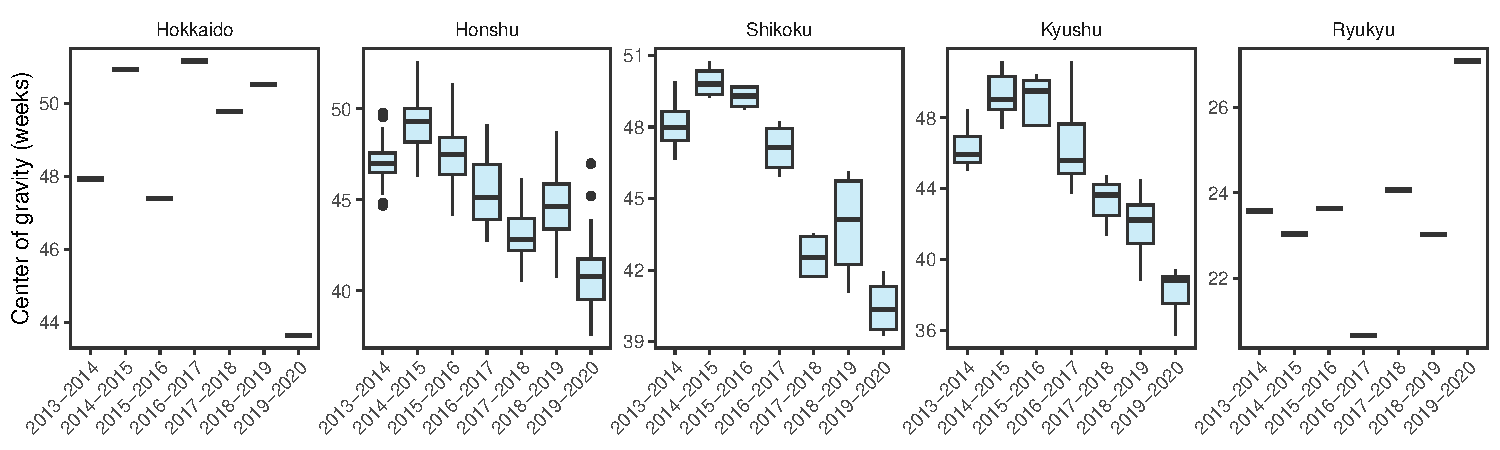
\includegraphics[width=\textwidth]{../figure/figure1_cog.pdf}
\caption{
\textbf{Estimates of center of gravity (i.e., the mean timing of an epidemic) across all prefectures, stratified by island.}
Hokkaido and Ryukyu islands each contain only one prefectures: Hokkaido and Okinawa, respectively.
The center (horizontal line), lower bounds, and upper bounds of the box plot correspond to median, lower quartile (25th percentile), and upper quartile (75th percentile), respectively.
The whiskers indicate the range of values that extend up to 1.5 times the interquartile range beyond the lower and upper quartiles.
Outliers, which fall outside this range, are plotted individually. 
}
\end{figure}



\begin{figure}[!pth]
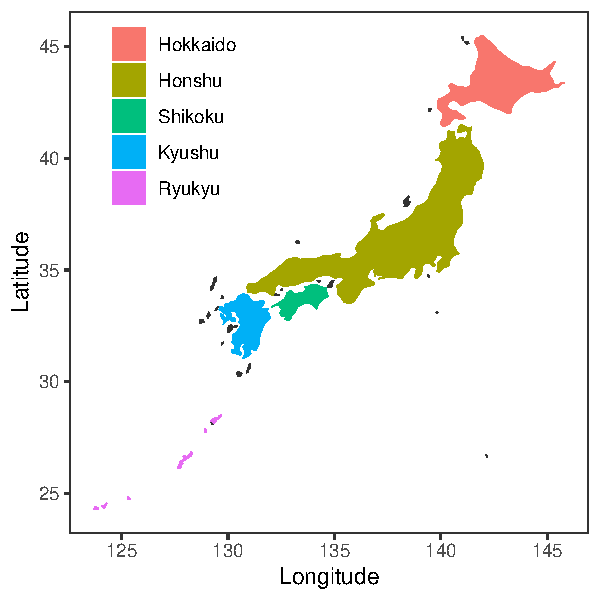
\includegraphics[width=\textwidth]{../figure/figure_map.pdf}
\caption{
\textbf{Colored map of Japan.}
Each of five major islands are marked by different colors.
}
\end{figure}

\pagebreak

\begin{figure}[!pth]
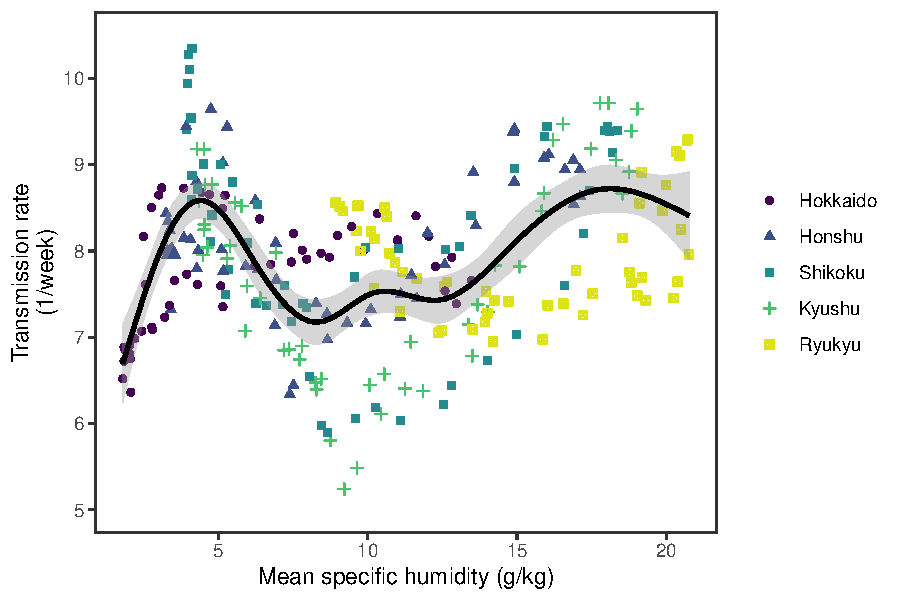
\includegraphics[width=\textwidth]{../figure/figure_joint_climate.pdf}
\caption{
\textbf{Joint relationship between the estimated periodic seasonal transmission rates and mean specific humidity across all five islands.}
Points represent the estimates across 52 weeks in each island.
The line represent a generalized additive model fit using cubic spline basis.
Shaded regions represent the corresponding 95\% confidence intervals (n=260).
}
\end{figure}

\pagebreak

\begin{figure}[!pth]
\includegraphics[width=\textwidth]{../figure/figure_comb_sirs_npi_temp.pdf}
\caption{
\textbf{Relationship between the estimated periodic seasonal transmission rates and mean temperature.}
Points represent seasonal transmission rate estimates across 52 weeks versus average humidity across 2013--2020.
Blue lines and regions represent the corresponding locally estimated scatterplot smoothing (LOESS) estimates and corresponding 95\%  confidence intervals (n=52).
Red lines and regions represent the corresponding quadratic regression fits and corresponding 95\% confidence intervals (n=52).
}
\end{figure}

\pagebreak

\begin{figure}[!pth]
\includegraphics[width=\textwidth]{../figure/figure_comb_sirs_npi_temp_hum.pdf}
\caption{
\textbf{Relationship between the mean weekly temperature and mean weekly humidity.}
}
\end{figure}

\pagebreak

\begin{figure}[!pth]
\begin{center}
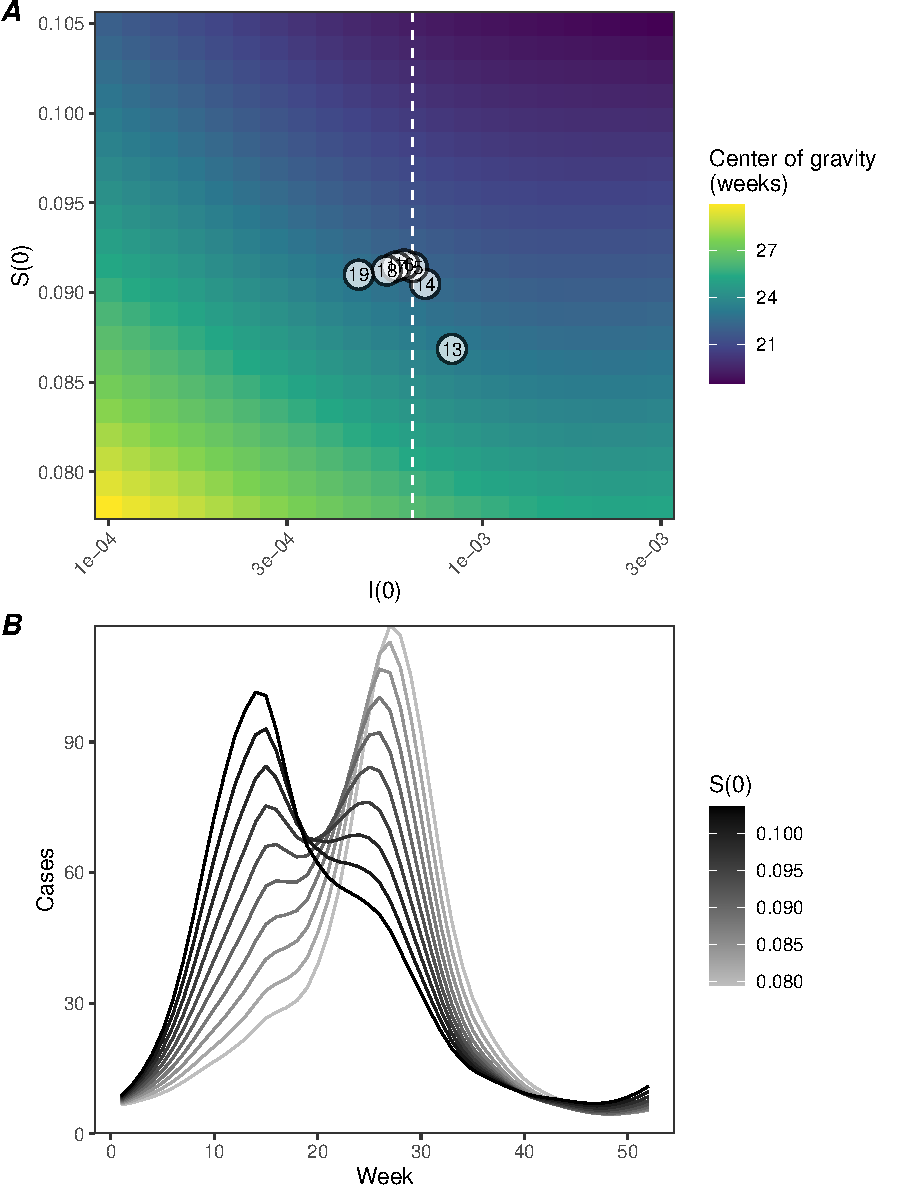
\includegraphics[width=0.8\textwidth]{../figure/figure_ryukyu_sirs_change.pdf}
\caption{
\textbf{A lack of increase in susceptible pool explains constant seasonality in Ryukyu island.}
(A) Predicted effects of the proportion of infected $i(0)$ and susceptible $S(0)$ at the beginning of season on center of gravity.
Points represent the estimated values for $i(0)$ and $s(0)$ between 2013 and 2019, showing the last two digits of a given year.
The white vertical dashed line represents the $i(0)$ value used for simulating epidemic dynamics in panel B.
(B) Changes in epidemic trajectories that would be caused by an increase in the susceptible proportion at the beginning of season for a fixed value of $i(0)$.
}
\end{center}
\end{figure}


\pagebreak

\begin{figure}[!pth]
\begin{center}
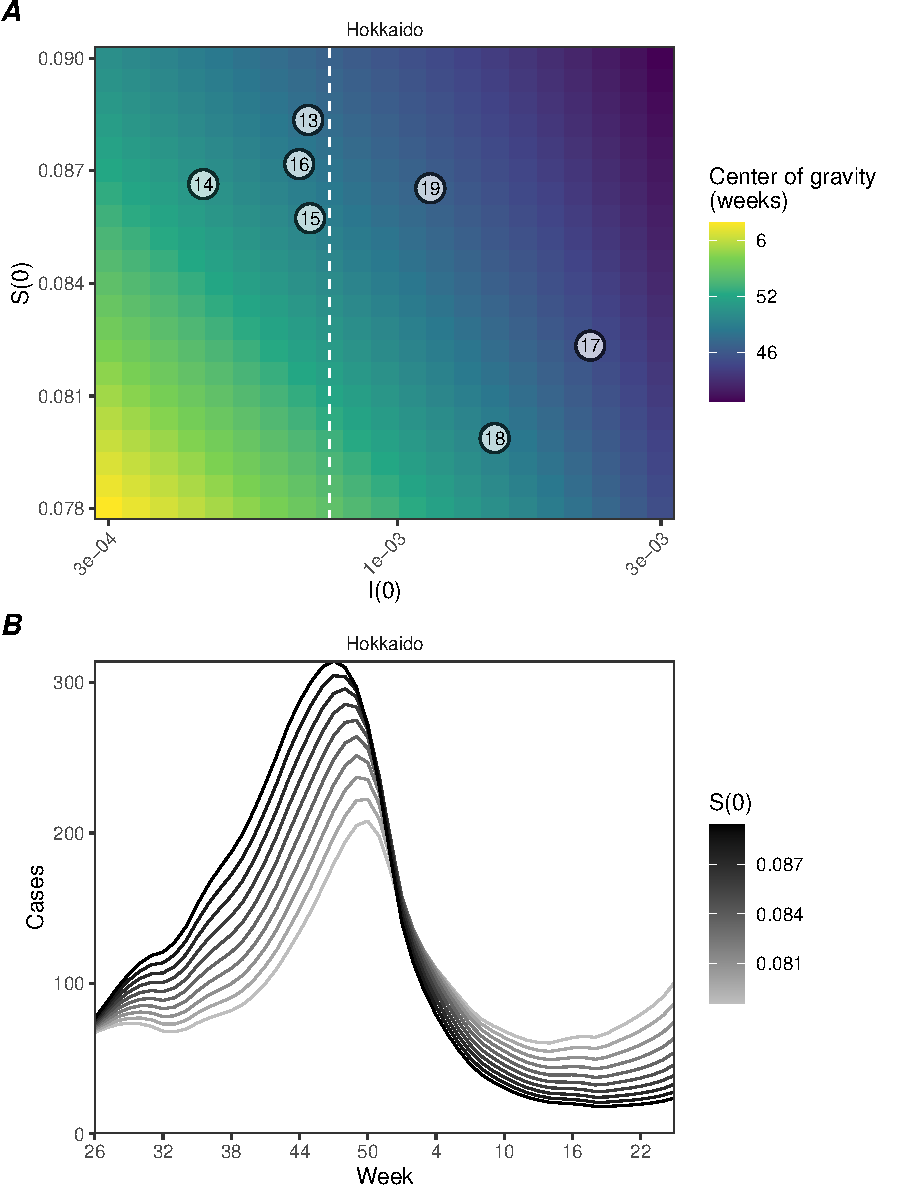
\includegraphics[width=0.8\textwidth]{../figure/figure_hokkaido_sirs_change.pdf}
\caption{
\textbf{Estimated change in susceptibility for Hokkaido island and counterfactual simulations assuming an increased susceptibility.}
(A) Predicted effects of the proportion of infected $i(0)$ and susceptible $s(0)$ at the beginning of season on center of gravity.
Points represent the estimated values for $i(0)$ and $s(0)$ between 2013 and 2019, showing the last two digits of a given year.
The white vertical dashed line represents the $i(0)$ value used for simulating epidemic dynamics in panel B.
(B) Changes in epidemic trajectories that would be caused by an increase in the susceptible proportion at the beginning of season for a fixed value of $i(0)$.
}
\end{center}
\end{figure}


\pagebreak

\begin{figure}[!pth]
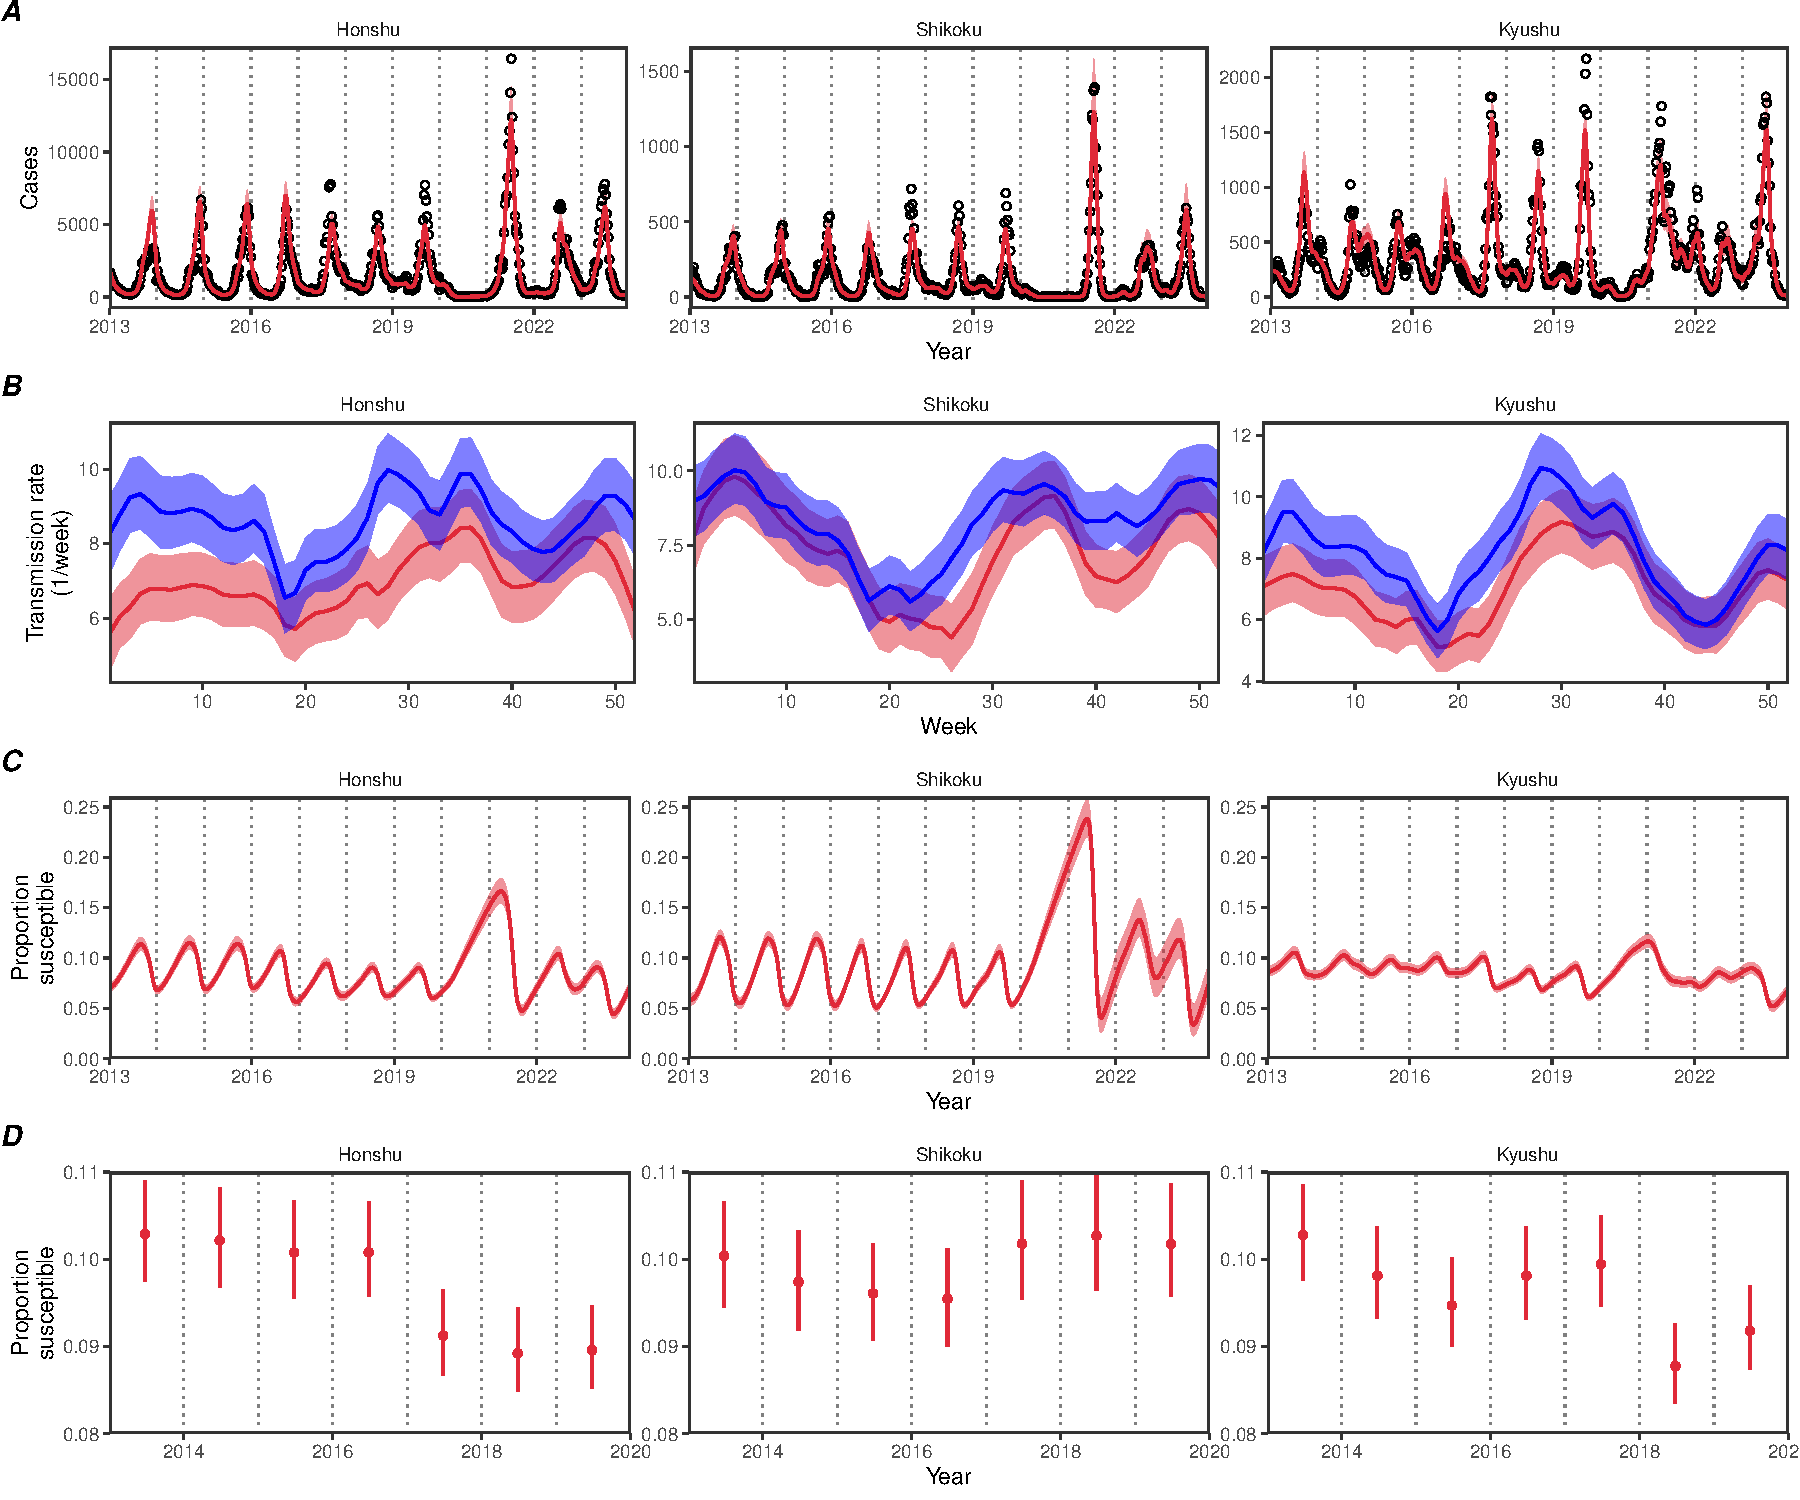
\includegraphics[width=\textwidth]{../figure/figure_comb_sirs_npi2.pdf}
\caption{
\textbf{Summary of SIRS model fits to RSV outbreaks across major islands in Japan.}
(A) Comparisons of observed cases (points) across the five major islands and fitted epidemic trajectories (red lines).
(B) Estimated periodic seasonal transmission rates before (red) and after (blue) the change in seasonality of RSV outbreaks.
(C) Estimated proportion of the susceptible pool over time.
In panels A--C, lines represent the estimated median of the posterior distribution (n=8000).
In panels A--C, shaded regions represent the 95\% credible intervals from the posterior distribution (n=8000).
(D) Estimated proportion of the susceptible pool on the 26th week of each year.
Points represent median from n=8000 posterior samples.
Error bars represent the 95\% credible interval in our estimates (n=8000 posterior samples).
}
\end{figure}

\pagebreak

\bibliography{perturbation}

\end{document}
